 
\chapter{Introductory}
\label{chap:introductory}
Prerequisites: calculus, biology

\section{Dynamical phenomenon}
\label{sec:dynamic-phenomena}

Generally speaking, a dynamical phenomenon is any process that instantly changes
over time. In that sense, a living cell is a dynamical process, with cell
growth, cell division, intracellular communication (like ion exchanges in
response to some cellular event), signal transduction, cell movement, etc. Even
though a single cell is a completed entity, it needs to use the energy and to
exchange matters (intake oxygen and expell wastes). Thus, a cell is not a closed
system. However, due to the fact that not everything can come into or expel from
the cells; cells are {\it selectively open
  systems}\footnote{ NOTE: the universe = the system + its surrounding

  + Isolated system = system that exchanges neither energy nor matter
  with its surroundings

  + Closed system = system that exchanges energy but not matter with
  its surroundings

  + Open system = it exchanges both energy and matter with its
  surroundings (such system takes in resources (energy, matters) from
  its environment, process them in some way, and produces output
  (energy, matters)). This concept is originally developed from
  thermodynamics.

  In real world systems, there is no complete isolated or closed
  system. Further, there is no true open system, but
  {\it selectively open system}. In other words, a selectively open
  system is, in need, open to some and closed to other influences.
  Cells have a mechanism to repel or digest strange particles, yet
  allow necessary particles (ions, \ce{CO2}...)  to get into the
  intracellular environment, i.e. the {\it cytoplasm}.  }.

Another unique characteristic of cells is that they are far from
{\it equilibrium}, if not never in equilibrium, i.e. there is always
influx and efflux of particles across the biomembrane.  We may be
interested in:
\textcolor{red}{what kinds of energies and matters does a cell
  accept?}
and
\textcolor{red}{from where do cells obtain these
  \hyperref[sec:resources-energy]{energies} and
  \hyperref[sec:resources-matters]{matters}?}.

\subsection{Resources of energy}
\label{sec:resources-energy}

Glucose \ce{C6H12O6} is an important energy source for cells in both
plants and vertebrates.
Plants obtain (radiant) energy from sunlight, i.e. photons which helps
making glucose, as given in the following equation
% \begin{center}
% \ce{6CO2_{(g)} + 12 H2O_{(g)} + photons ->[\text{enzyme}] C6H12O6_{(aq)} + 6O2_{(g)} + 6H2O_{(1)}}
% carbon dioxide + water + light energy \ce{->} glucose + oxygen + water
% \end{center}

\begin{center}
\ce{ $\underset{\text{carbon dioxide}}{\ce{6CO2_{(g)}}}$ +
$\underset{\text{water}}{\ce{12 H2O_{(g)}}}$
 + $\underset{\text{light energy}}{\text{photons}}$ ->[\text{enzyme}]
$\underset{\text{glucose}}{\ce{C6H12O6_{(aq)}}}$ +
$\underset{\text{oxygen}}{\ce{6O2_{(g)}}}$ + 
$\underset{\text{water}}{\ce{6H2O_{(1)}}}$
}
\end{center}


Unlike plants, vertebrates don't have the proper enzymes to enable
the glucose synthesis from sun light. Thus, they obtain energy
(nutrients) from foods in a process known as {\it metabolism process}
whose reactions are called {\bf metabolic reactions}
(Sect.\ref{sec:metabolic-reactions}).

\subsection{Metabolic reactions}
\label{sec:metabolic-reactions}
\label{sec:anabolic-reaction}

There are two
classes of metabolic reactions\footnote{\url{http://www.scienceclarified.com/Ma-Mu/Metabolism.html}}:
{\it catabolic reactions} and {\it anabolic reactions}.
\begin{itemize}
\item In the catabolism process (Sect.\ref{sec:catabolic-energy-metabolism}),
  complex molecules from foods, with the support of enzymes, are broken down
 into simple molecules and releases energy. 
  
  The total amount of simple molecules is called {\it metabolic pool}.

\item In the anabolism process, the released energy from catabolism
  process is used to build other complex molecules
  (i.e. biomolecules), or for other purposes 
(e.g. keeping body warm). 

The remaining unused energy are stored in the body for later use in the form of
ATP (Sect.\ref{sec:ATP-synthesis}) or fat
\footnote{\url{http://www.scienceclarified.com/Ma-Mu/Metabolism.html}}.

\end{itemize}

\subsection{Resources of matters}
\label{sec:resources-matters}

At the macro level, the resources of matters that plants need are
photons, \ce{CO2}, \ce{H2O}... and vertebrates need are various kinds
of nutrients in the form of food, beverages...  The constituents of
nutrients can be
\begin{enumerate}
\item
  carbohydrate\footnote{carbohydrate is a compound consisting of
    carbon, oxygen, and hydrogen} $\rightarrow$ sugar
\item lipids $\rightarrow$ fatty acids, glycerol
\item proteins $\rightarrow$ amino acids
\end{enumerate}


At the micro level, we're focusing on how and what a cell exchanges to
each other and to extracellular environment. Matters that cells
exchange to each other and to extracellular environment can be ions
(\ce{Ca^2+}, \ce{K+}, \ce{Na+}...), proteins and some other substances
whose amount can vary depending upon the {\bf state} of the cell.

A cell, as a dynamical system, is modeled to undergo through a number of
different states. How the state of a cell is defined varies depending upon how
detailed of the cell we want to model. Normally, the state of a dynamic model is
represented in a qualitatively way by a set of {\bf state functions}
(Sect.\ref{sec:state-functions}).
This will be covered in the next section. % Here, we meet the concept of state.

\section{Mathematical biology: Computational modelling in biology}
\label{sec:comp-modell-biol}

This book will introduces different useful computational models, and how to
develop a good one, starting from models for different types of cellular
components (e.g. ion channels, pumps, exchanger) from asbtract level to mechanistic level,
and then at the whole cell level, which we target electrical excitable cells for
the heart and the brain.

{\bf Mathematical biology}, the branch of math applied in biology, is
a strong and well-developed branch of applied mathematics.  Let's
review

\begin{enumerate}
\item  {\it why we need a model}?
  \begin{itemize}
  \item all quantities of interest cannot be measured {\it in
      vivo}.
    Some of these can be obtained {\it in vitro} on small tissue
    preparation or isolated cells.

  \item the ultimate purpose is to study the dynamics of the whole
    cells, not just a part or a small cell of it.

  \item computer simulation, {\it in silico}, can yield the hidden
    information that we cannot obtain from {\it in vivo} or
    {\it in vitro} measures.
  \end{itemize}

\item {\it What is a good model}?
  \begin{itemize}
  \item a too simple model fails to capture the salient behavior and
    have limited predictive capability

  \item a too complex model can be computationally intractable.

  \item a good model depends on the questions being answered.
  \end{itemize}
\end{enumerate}

\subsection{Challenges in computational biology}

To study a dynamical system (Sect.\ref{sec:dynamic-phenomena}), i.e.
understanding the dynamic of the system, we need a means to record how the
system changes over time.

To observe the changes from a real system, in laboratories, data are record
periodically. This is not a trivial task as in nature, even the simplest dynamic
phenomena are exceedingly complex, especially in molecular processes.
For example, in many problems, it's not easy to follow the changes due to the
tiny time scale (i.e. the temporal resolution of the recorder is not high
enough) or the signal is too small (i.e. the spatial resolution of the recorder
is not high enough) or due to the rareness of the event (i.e. it may take months
or years for a change to happen).

Given that challenges, computational modelling aims at deriving the systematical
change of a system based on the experimental data.  Even though computational
models will never be as useful as laboratory data in terms of providing a
concrete view about a physiological process, it does provide a quantitative
understanding where conducting an experiment is very expensive or hard to do. As
one said: there is no accurate models, but there are useful models.

A good model can reproduce experimental data that were used to create them.
However, a useful model is not only a good model, but is also capable of
predictive. That is, they can be used to guide making decision in hypothesis
testing, medical treatment, or in drug developments.
Useful models need to be designed following closely with experimental data,
using some mathematical formulations to describe the dynamical process
(Sect.\ref{sec:dynamic-phenomena}).

Before we can develop such models for a particular problem domain, we need to
understand how to represent a dynamical system
(Sect.\ref{sec:representing-system}).

\subsection{Representing a system: state functions, state space}
\label{sec:representing-system}
\label{sec:state-functions}
\label{sec:state-space}

A system can be studied when it reaches the steady state condition. To gain the
maximal control of the system, and to avoid any undesired affects, such a system
is often examined with the assumption of a {\bf conserved system}, i.e. by
disturbing a little bit the parameter, the system go through a number of change
but no loss in energy. Thus, the change in the system can be considered as going
through a number of reversible steps. Sect.~\ref{sec:reversible-vs.-non} will
discuss why the assumption of a reversible system is important.

% After reading the previous section, we now agree that cells are dynamic.
From the view point of thermodynamics, a dynamical system can be uniquely
determined throught its current state.
Thus, to study the behavior of a dynamic phenomenon, it's important to know the
{\bf states} of the process/system/phenomenon at different time points. This
state is often determined by a set of parameters whose values do not depend upon
how the system reaches that state. It means that the values of such parameters
are functions of state; i.e. a parameter is called a {\bf state function}
\footnote{Read ThermoStat book, Chapter 5 (Thermodynamics System-State) for more
detail}.

\begin{mdframed}
  
  In a thermodynamic system, there are many quantities that are
  considered as state functions: pressure ($p$), volume ($V$),
  temperature ($T$), internal energy ($U$), mass ($m$), energy ($E$),
  Helmholtz free energy ($F$ or $A$), Gibbs energy ($G$)\footnote{The word
  ``free'' in Gibbs free energy was banished since 1988 by IUPAC},
  entropy ($S$), enthalpy ($H$).
  Among them, {\it Gibbs (free) energy function} is the most important and the
  most widely used. % So, by using a subset of such quantities, we can
  % fully describe a system.
\end{mdframed}

The smallest set of state functions that can fully characterize a system forms
the {\bf state space} of that system; and its size is called the {\bf dimension}
($D$) of the state space of the system. It's important to know that this set is not
unique and the choice a specific state space varies from problem to problem. 

{\bf Example}: a system of monatomic gas with a fixed number of particles has $D
= 2$, i.e. the system is uniquely determined by 2 parameters. The two widely
state spaces are (1) $V$ and $T$; (2) $T$ and $p$. In essence, the two state
spaces ($p,T$) and ($V,T$) are equivalent, and simply form two different
coordinate systems on which we can study the dynamics of the system.

If we assign an energy level with each state, the set of all states can form one
or more energy wells (or potential wells). A state of a dynamical system can be
stable and unstable; and those with energy at the bottom of the energy wells are
stable states. As a dynamical system, the system can change from one state to
another, in a reversible or irreversible way.

With the current limitation of mathematical tools, we can only study a dynamical
system (i.e. examine the values of the state functions) under the assumption of
stable state or equilibrium state, from where we can assume any pertubation is a
reversible process (Sect.\ref{sec:reversible-vs.-non}).
% \textcolor{red}{As a matter of fact, the condition of equilibrium is very
% important in studying the dynamics of a system using computational tools}. In
% the next section, we'll discuss why the assumption of reversible is important
% and how to represent a dynamical system to study at equilibrium state
% (Sect.\ref{sec:reversible-vs.-non}).
  
\subsection[Quasi-statics vs. Reversible vs. Non-reversible]{Quasi-statics vs.
reversible vs. non-reversible systems}
\label{sec:reversible-vs.-non}

The condition of equilibrium is very important in studying the dynamics of a
system using available computational tools (Sect.\ref{sec:repr-dynam-syst}).

{\bf Why can't we study an irreversible process and if we have
  reversible process, how can we study it?}
- In a non-reversible system, the amount of work that we actually get out of the
system is always less than the input energy and the amount of useless energy
depends upon how the system was designed and the material involved. To take into
account the loss, we may need to incorporate the entropy into the simulation
(Sect.\ref{sec:entropy}).
Also, calculus cannot be used; since measurable steps are not in uniform
infinitesimal jumps.  So, it's hard to study such systems and compare them using
our current available computing power as well as mathematical language.

As a matter of fact, we mainly study the dynamics of a closed system under the
``reversible'' assumption. In such idealized system, there is no energy loss,
i.e. no entropy. Thus, in a small enough time interval, the change is considered
ideally {\it
  reversible}\footnote{An irreversible process occurs in certain direction. Once
  the process having been taken place, the system cannot go back to its previous
  state. A reversible process is a process that can be reversed without leaving
  any trace during its change. In practice, a truly reversible process does not
  exist. The real process are irreversible}.
A reversible process can be represented by differential equations to derive the
results and these results are independent of the materials used to construct a
particular system. The widely mathematical tool to study such systems is
calculus (ODE and PDE) - Sect.\ref{sec:repr-dynam-syst}.


\begin{figure}[hbt]
  \centerline{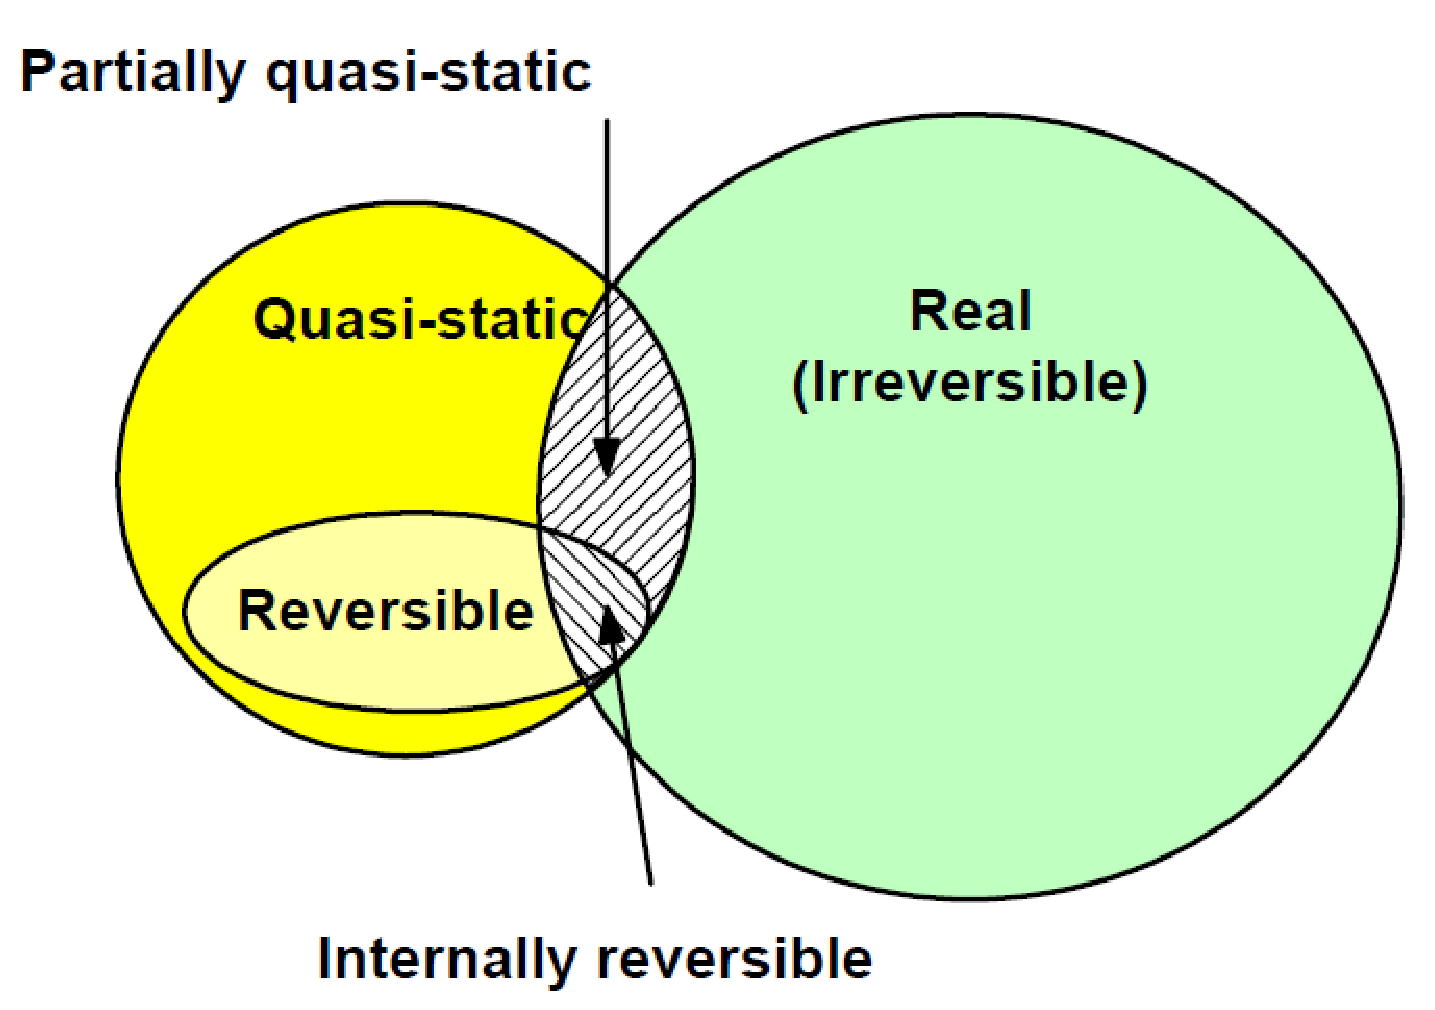
\includegraphics[height=5cm,
    angle=0]{./images/internal_reversible.eps}}
\caption{Internally reversible}
\label{fig:int_reversible}
\end{figure}

A reversible system can be
\begin{itemize}
\item externally reversible: the reversible process occur outside the
  system
\item internally reversible: the reversible occur inside the system
\item totally reversible: the reversible occur both inside and outside
\end{itemize}
\textcolor{red}{We'll make use only ``internally reversible process''}
in which the system pass through a series of equilibrium states and
can return to the initial state on exactly the same set of equilibrium
states, with the reverse
order\footnote{Fundamental of thermo-fluid sciences. Yunus A. Aengel,
  Robert H. Turner, pg.246}. A reversible process is in {\bf quasi-static}, i.e.
  each state is infinitesimally close to equilibrium (NOTE: A quasi-static process
  can be irreversible). By examining the system in a series of equilibrium
  states, the values of state functions can be estimated as the time evolution.
  As the process remain arbitrarily close to equilibrium at all time, the time
  evolution of a quantity is represented by differential equations.


% \subsection{Example 1}
% \label{sec:example_1}

\subsection{Representing (the dynamics of) a reversible system: ODEs, PDEs}
\label{sec:repr-dynam-syst}

The widely used method to represent the change of a {\it reversible system}
(Sect.\ref{sec:reversible-vs.-non}) during the time evolution is using
mathematical formulas. In mathematical language, a small change of a quantity
over time is represented in the form of {\it differential equations}, e.g. ODE
or PDE. The system can be solved using {\it deterministic} or {\it stochastic}
models.

In deterministic models, the assembled behavior of the system is assumed, i.e.
we always get the same result at different trials for a given input. In many
cases, practically, it's important to incorporate the stochastic behavior of the
system. Thus, the role of stochastic modelling is getting more important; yet
require more computational time.


\subsection{Kinetic scheme}
\label{sec:kinetic-scheme}


\begin{framed}
  We use the term {\bf mechanism} to refer to how an event occurs in a
  physical system; while the term {\bf kinetics} refers to how an event occurs
  from the mathematical model. For example: the excitation-contraction coupling
  mechanism or the kinetics of channel gating in a Markov-Chain model.
\end{framed}

Kinetic schemes focus attention on conservation of material (in a closed set of
reactions, material is neither created or destroyed) and flow of material from
one state to another (Sect.\ref{sec:kinet-interpr-ionic}).
\begin{itemize}
  \item a set of states
  
  \item arrows connecting one state to another
\end{itemize}

The notion of "state" is context-dependent: it may mean actual material quantity
of a molecular species (sometimes moles, sometimes mass), the well-stirred molar
concentration in a volume or the density on a surface, or the probability of a
particle being in a particular state.
\begin{itemize}
  \item  "the value of state A" we mean a value expressed in the dimensions of
  A. When A is in units of concentration or density,

  \item "the material in state A" is the product of A and the size of the
  compartment (volume or surface) in which A is distributed.
\end{itemize}

In a kinetic scheme, arrows that point toward or away from a state represent
paths along which material enters or leaves the state.
For each state there is a differential equation that expresses how the amount of
material in the state is affected by fluxes that enter and leave it.

As a result, any kinetic scheme is easily translated into a corresponding set of
differential equations (Sect.\ref{sec:repr-dynam-syst}). 


\subsection{Steps to build a mathematical model}
\label{sec:mathematical-biology}


In practice, no mathematical model can produce the result identical to the
system it modeled.  In stead, it is a simplification of the real system, and
typically in a smaller scale. Nevertheless, a model can be practicable if (1)
its behavior show the trend of what's going on as closed to that of the real one
as possible, (2) its behavior/change is tractable (using analytical methods or
numerical methods).

Thanks to the abundant availability of quantitative experimental data,
and the rapidly development of computing power, computers have proved
to be a powerful tool to dissect the molecular processes.  A
mathematical model solved on computers is called the
{\bf computational model}.  Below is the logical steps to create a
computational model using computers.

\begin{enumerate}
\item Taking clues from the experimental data \ce{->} try to identify
  the {\it biological/molecular mechanism of the dynamic phenomena}
  from data/plots (this may require closed consultants with
  experimentalist working on the problems.), the pathways (which one
  interact with which one, which one induce the
  activation/inactivation of which one, etc.)

\item {\it Derive a hypothesis} (an overall model) using arrows given in
  Fig. \ref{fig:pathway-key} \ce{->} we call this schematic
  representation, or cartoon, which should be explicitly clear enough
  to be translated into a series of elementary steps representing
  individual mechanisms.


\item Apply the basic laws of physics and chemistry to translate the
  elementary steps of the molecular mechanisms into a mathematical
  expression.

\item The changes based on the mathematical expressions are then expressed in
the form of time dependent differential equations (Ordinary Differential Equation
  (ODE) or Partial Differential Equation (PDE)).


  \textcolor{red}{``How can a system be represented in ODEs?''}  - when
  the system is broken into individual components, as well as
  corresponding quantities for each components, the changes in such
  quantities (i.e. dependent variables) can be represented using
  ordinary differential equations $dX/dt=f(X,Y,...)$.

\item Solve the equations using some standard numerical methods (e.g. Euler
method, Runge-Kutta method) or, in simple cases, analytical methods.

\item {\it Hypothesis testing} \ce{->} finally, carefully study the
  differential equations to know whether the overall model is correct
  or not (by comparing the numerical solutions with some given
  experimental data).

\end{enumerate}

{\bf IMPORTANT}: Rigorous analysis of complicated (ordinary/partial)
differential equations requires specialized training, since there are
many subtleties that can be gained only with experience.

To support the interpretation of the problem, a {\it kinetic diagram}
should be utilized. In this diagram, it should

\begin{itemize}
\item for each component:
  \begin{enumerate}
  \item identify all {\bf dependent variables}, i.e.  changing
    quantities of the component. These quantities are normally state
    functions. Typically, in cellular physiology, the state functions
    of interest are the ion concentrations ([\ce{Ca^2+}], [\ce{K+}],
    [\ce{Na+}], [IP3]...). We may also investigate the fraction of ion channels
    in a particular state (Open or Closed).
  \item list all possible
    {\bf transfers between every pair of variables} and adopt a symbol
    to represent a {\it rate constant} associated with each transfer;
    then estimate the values of the rate constants. 
    
    If everything is unchanged, the rate constants are always constant. However,
    due to the dynamics of the internal media inside the cell, such rate
    constants can be functions of something else (the conditions under which we
    perform the measurement). Thus, we need to predict the functional form of
    the rate constants, and then calculate it based on given values.
  \end{enumerate}

\item inter-components:
  \begin{enumerate}
  \item identify all {\bf constraints}, and make sure the system is
    closed (solvable) based on {\bf conservation laws}. 
    
  \item between two components, there can be more than one parameter to
    change, so there can be more than one connection between them. 
  \end{enumerate}
\end{itemize}

{\bf Example}: A cell is composed of different components:
mitochondria, sarcoplasmic reticulum (SR), Golgi apparatus, cytoplasm,
nucleus...

The problem will be more complicated if the change in one parameter is
dependent upon the change in the other ones, e.g. $\dot{X_i} = f(X_i,
X_j, X_k...)$.  In almost practical systems, finding $X_i(t)$ can only
be done using numerical methods. However, there are some cases the
system can be solved analytically.

\section{Numerical issue when solving a computational model}

Computers are powerful machines to help solving complicated problems.
However, they do not have infinite precision. Therefore, knowing about errors is
important in choosing the right numerical methods, and data types to represent
the independent variables.

\subsection{round-off error: machine + language dependent}
\label{sec:round-off-error}

To study the time evolution of a dynamical system, we do integration of the
dependent variables using computers. As we cannot represent a real value on
computer with infinite accuray, there's always a {\bf round-off error}. You can read
more how a numerical value is represented on computer elsewhere [REF].
It means that the value stored on computer is an approximate to the true value. To reduce this
error, we can use more bits in the decimal parts, e.g. from single precision
(4bytes) to double precision (8bytes). 

On every computer, for each data type, there's a smallest representable number,
called $\eta$, so that when a number of order unity is added to $\eta$, the
result is a new number of different value. The value of $\eta$ is depending how
many bytes is used to represent the value. So, the round-off error is denoted as
$\bigO(\eta)$.

For IBM-PC, and double-precision, $\eta=2.22\times 10^{-16}$ (which is specified
in the system header file \verb!float.h!).
\begin{verbatim}
#define __DBL_EPSILON__    2.2204460492503131e-16
#define __FLT_EPSILON__    1.19209290e-7F
\end{verbatim}
In Fortran, the intrinsic function EPSILON(X) return the $\eta$ value, of the
same kind as X, so that $(1+\eta)$ is the smallest number that is greater than
1.

\subsection{truncation error (per time-step): numerical method dependent}
\label{sec:truncation-error}

Computer is useful in representing the mathematical formula in the form of
linear or non-linear algebraic equations.
A powerful mathematical tool to approximate an arbitrary function f(x) in the
form of algebraic equations is {\bf Taylor expansion} which can be of different
order of accuracy to the original formula. The error is called {\bf truncation
error}.

Depending on the order to keep, we'll have different magnitude of truncation
error. The equation for the line is derived from Taylor expansion of the curve
\begin{equation}
y(t_n+h) = y(t_n)+ y'(t_n)h + y''(t_n)\frac{h^2}{2} + \ldots
\end{equation}
or
\begin{equation}
\label{eq:Taylor_2nd_order_form}
y_{n+1} = y_{n} + f(t_n, y_n) h + \bigO(h^2)
\end{equation}

As the form being solved by the computer (e.g.\ref{eq:Taylor_2nd_order_form}) is
an approximateion of the original equation, this is another source of error,
called {\bf truncation error} which comes from the numerical method being used.
The higher the order of $\bigO(\cdot)$, the smaller the truncation error. In
ODE, we typically try to reaches at least, second-order in time $\bigO(\Delta
t^2)$. In PDE, it's very challenging to get second-order in both space
($\bigO(\Delta x^2)$, $\bigO(\Delta y^2)$, \ldots) and in time 
$\bigO(\Delta t^2)$, with good speed performance.


\subsection{accumulative error (net truncation error)}
\label{sec:accumulative-error}
\label{sec:net-truncation-error}

In solving ODE, Euler method is the first-order approximation of the
unknown curve $y(t)$ from point of time $t_1$ to $t_2$. 
Using the initial value $y_0$ and the first-order appximation Euler method, we
have
\begin{equation}
\frac{dy}{dt} = y'(t) \approx \frac{y_{n+1}-y_n}{h} 
\end{equation}
we can find $y_{n+1}$ with the truncation error is $\bigO(h^2)$ with $h$ is the
step length. The shorter the step length, i.e. $h=t_2-t_1$, the more accuracy
the result. On an interval of unity length, with step length $h$, the number
of steps is $h^{-1}$. So, the accumulative error (or net truncation
error) is $\bigO(h^2) \times h^{-1} = \bigO(h)$. In other words, the
accumulative error using Euler method to do the integration is proportional to the step-length. 

In essence, it's important to choose an appropriate numerical method to limit
the cumulative relative error to a small enough value. Suppose we want the
cumulative error below $10^{-6}$, so we need at least 1 million time-step per
unit time interval in $x$.
 
\begin{framed}
A method is $n$-th order if the truncation error {\it per step} is
$\bigO(h^{n+1})$.
\url{http://farside.ph.utexas.edu/teaching/329/lectures/node33.html}
\end{framed}

\subsection{net round-off error}

Assuming that each time step has only one floating-point operation, then the net
round-off error, with $\eta$ is the round-off error per arrithmetic operation
and $h^{-1}$ operations. Then the total round-off error is $\eta/h$, after
$h^{-1}$ iterations.

\subsection{total error: net round-off + net truncation errors}
\label{sec:total-error}

So, the total error is the sum of the net round-off error and net truncation
error. 

Example: for Euler method is
\begin{equation}
\epsilon = \eta/h + h
\end{equation}
So, truncation error dominates at large time-step while round-off error
dominates at small-time step. The minimum value of this net error is
$\epsilon_0 \approx \eta/2$ when $h = h_0 \approx \eta^{1/2}$. 

\subsection{choosing time-step: ODE}

As discussed above, there's no point in making the time step smaller than
$h_0 \approx \sqrt{\eta}$.

So, at the double-precision,
i.e. $\eta = 2.2\times 10^{-16}$, we don't need to use time-step smaller than 
$h_0 = 10^{-8}$ which gives $\epsilon_0 \approx 10^{-8}$. This level of accuracy
is good enough for most  scientific calculations. 

\begin{framed}
For single precision, where $\eta = 1.19\times 10^{-7}$, the practical
smallest time-step is $h_0\approx 3\times 10^{-4}$ and net error $\epsilon
\approx 3\times 10^{-4}$ which is not adequate for scientific calculation. 
\end{framed}

Now, we come to the question what is the largest time step we can use.
Using large time-step, we have large truncation error, or we call it {\it
numerical instabilities} where the total truncation error explodes along the
course of the simulation.

For other methods of higher order accuracy, we can use a larger time-step. 

\subsection{choosing time-step and space-step: PDE}


Check more: 
\url{https://en.wikipedia.org/wiki/Linear_multistep_method}
\url{https://en.wikipedia.org/wiki/Courant-Friedrichs-Lewy_condition}
% TODO: Update this part (critical time-step and spatial step)

This paragraph tells us the choice for step in space and time. In Euler method
to solve PDE the choice is often
\begin{verbatim}
1-Dimension: D*h/(dx^2) < 1/2
2-Dimension: D*h/(dx^2) < (1/2)^2
3-Dimension: D*h/(dx^2) < (1/2)^3
\end{verbatim}
with $D$ is Diffusion constant. 

\subsection{choosing time-step: dynamics}

A dynamic time-step numerical methods are also good
choices. 


% \section{Kinetics of a chemical reaction}
% \label{sec:basic-equat-react}

\section{An example of a dynamical system: a simple model of ion channel gating}
% \label{sec:math-model-cell}
% \section{}
\label{sec:model-ion-channel}


In Sect.\ref{sec:comp-modell-biol},, we have learnt different factors that
determine the properties of a system as a number of states, and essential
concepts of state transition similar to a chemical reaction. In this section, we
will apply those knowledge, especially the 6 distinct steps in section
\ref{sec:repr-dynam-syst}, to the dynamics of a simple system of $N$ ion
channels. Each channel is assumed to be in either Open or Closed state.

\begin{framed}

  All matters are exchanged in cells via tiny gates formed by special proteins
  known as channels.  The term ``gating'' refers to the opening/close (or
  activation/deactivation) of a class of ion channel\footnote{an ion channel is
  a gate that allows only ions to go through}. An example is the glucose protein
  (GLUT) with two states in an oxidized cholesterol bilayers, as shown in
  Fig.~\ref{fig:ionchannel}.
  In some complicated models, the gating can be modelled with more than two
  states, e.g. Close, Inactive, Open.
\end{framed}

\begin{figure}[htb]
  \centerline{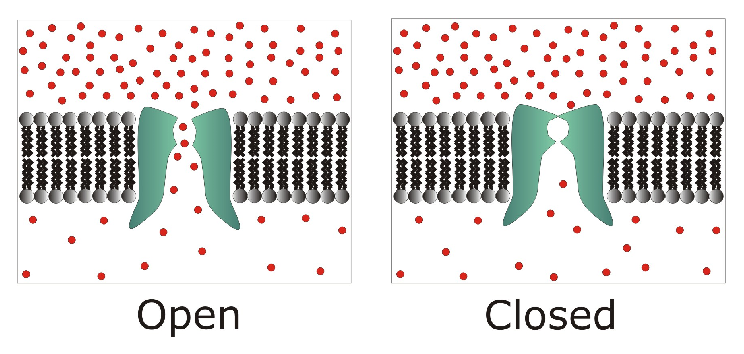
\includegraphics[height=3cm]{./images/ion_channel_state.eps}}
  \caption{A two-state model of GLUT ion channel (Open=conducting state,
  Closed=inactive)}
  \label{fig:ionchannel}
\end{figure}

% We assume a system of 2 states; and the transition between open and
% close is random, and is independent from any external factors.

\subsection{Assumptions}

\begin{enumerate}
  
  \item The system is a conserved system: i.e. 
  
  \begin{itemize}
  
    \item the number of channels is fixed. At a time, there is $n_1$ Open
    channels and $n_2$ Closed channels, and $N=n_1+n_2 =$ constant.

For simplicity, \textcolor{green}{we assume that there is only one type of ion
channel in a single cell (so they all have the same kinetics, i.e.
same transition rates)}\footnote{However, in a practical application, varying
number of channels was neccessitated by birth or death of channels during the
course of a {\bf long} experiment}.
  
    \item and the total number of ion channels is fixed.
  \end{itemize}
  
  \item The transition from one state to another can be represented in the form
  of the kinetic diagram which denotes the transitions between 2 states by solid
  lines and arrows
  \begin{equation}
    \label{eq:7}
    \ce{C <=>[k^+][k^-] O}
  \end{equation}
  with C denote ``closed'' state, O denotes ``open'' state.  $k^+,
  k^-$ are {\it rate constants} (like those described in a chemical
  reaction) and the arrows represent the
  {\it elementary molecular processes}.

  Further, it's important to know that this is a reversible and
  unimolecullar process in the sense that only a single reactant
  (NOTE: bimolecular process when there is two reactants). 

\end{enumerate}


% \item The biological mechanism is the switching between 2 states of an
%   ion channel, as shown in Fig.\ref{fig:ionchannel}. A single channel
%   is considered as the atomic component, so there is no need to break
%   the system into subproblems.
% 
% \item Derive an overall model: the model is 
\begin{framed}
  
  
  \textcolor{red}{How we define the measurement of ``concentration''?}.
  For a comprehensive references of different way to define
  ``concentration'', read
  \href{http://en.wikipedia.org/wiki/Concentration}{[wiki]}. Here are
  some examples:

  \begin{enumerate}
  \item If channels are in intact cells, concentration is often
    expressed in terms of volume-volume percentage.

  \item Another common use measurement is expressed in terms of the
    total weight of integral membrane protein in a sample

  \item For ion channels in a single cell, concentration can be
    expressed in terms of the fraction of ion channels in that
    state.
  \end{enumerate}

\end{framed}

As O and C are not chemical compounds, we cannot use the mass-mass
ratio as the measure of concentration. In our problem, we choose (3)
as the definition of concentration of ion channels. 
% Given that $N$ be
% the number of ion channels in the cell membrane and it is large
% enough. 
% 
% At time $t=0$, $N_0$ be the number open ion channels and $N_1$ be
% the number of closed ion channels. Then, we have

\begin{equation}
  \label{eq:9}
  [\text{O}]_0 = f_O(t=0) = \frac{N_O(t=0)}{N}, [\C]_0 = f_C(t=0) =
  \frac{N_C(t=0)}{N}
\end{equation}
To study the system, we need to know how $f_O(\cdot)$ and
$f_C(\cdot)$ change over time.

\begin{mdframed}
Since our kinetic model involves only 2 states $\{O,C\}$, and no
birth/death, we always have $N = N_0(t) + N_1(t)$=constant or 
$f_O(t) + f_C(t) =1$. 
This satisfies the idea of conversation law which physically
states that ion channels are neither created nor
destroyed.
\textcolor{red}{The assumption of conservation of the quantities in
  a system is critical to the simulation study of the system}.
\end{mdframed}

\subsection{Flux and Concentration: Mathematical abstraction of the real system}
\label{sec:flux-example}
\label{sec:concentration-example}



The {\it rate of transition} $J$, also referred to as {\bf flux}, in which ion
channels turn from one state to another at a unit of time is used
(Sect.\ref{sec:fluxes}).
    
Apply the basic law of physic and/or chemistry:
  \begin{itemize}
  \item flux from C to O: the rate of of channels swtiching from closed state to
  the open state per a unit of time is
  \begin{equation}
  J_+ = k^+[\C]
  \end{equation} 
    
    
   \item flux from O to C: the rate of transition in which ion channels turn
   from the open state to the closed state per a unit of time is
    \begin{equation}
    J_- = k^-[\text{O}]
    \end{equation}
\end{itemize}

If we assume the total amount of channels is large enough and the assumption
that total ion channels is fixed, then the amount of channels in each state, say
open and closed, can be represented in the form of {\bf concentration} or the
fraction of channel in that state (Sect.\ref{sec:concentration}), denoted as [O]
and [C] respectively.

Using the {\bf law of mass action} (Sect.\ref{sec:law-mass-action}, we obtain
the {\it reaction quotient} Q
    \begin{equation}
      \label{eq:8}
      Q = \frac{[\text{O}]}{[\C]}
    \end{equation}
By comparing the value of Q with the equilibrium constant $K_{eq}$, it can tell
us whether the reaction moves to the right ($Q<K_{eq}$ or left direction ($Q>K_{eq}$).

\subsection{ODE: first-order kinetics representation of the model}
\label{sec:first-order-kinetics-example}

To study a dynamical system, i.e. the change over time, the available tools from
maths are ODE or PDE (Sect.\ref{sec:repr-dynam-syst}).

From time $t_1$ to $(t_1+\Delta t)$, the number of open channels can change,
as do the closed channels. We have
\def\flux{{\text{flux}}}
\begin{equation}
  \begin{split}
    \label{eq:10}
    \flux_{O \ce{->} C} &= J_- = k^- f_O  \\
    \flux_{C \ce{->} O} &= J_+ = k^+ f_C = k^+ (1-f_O)
  \end{split}
\end{equation}
with $k^+, k^-$ are the rate constants, and
the concentrations are $f_O, f_C$ respectively at each side of the
reaction.

The degree of freedom of the system is 1. So, if we know the number of
opened channels at a time instant, it can tell the fraction of closed
channel. So, to study the system, we only need to use a single ODE for
$f_O$
\begin{equation}
  \label{eq:11}
  \frac{df_O}{dt} = - J_- + J_+  =  - k^- f_O + k^+ (1-f_O)
\end{equation}

\textcolor{red}{For simplicity in notation, we use $f$ to substitute
  for $f_O$ with $f$ is a function of time, $f(t)$}.
\begin{equation}
  \label{eq:254}
  \frac{df}{dt}  =  - (k^-+ k^+) f + k^+ =  - (k^-+ k^+) (f - \frac{k^+}{k^-+ k^+})
\end{equation}


% Using mathematical equations to represent the change of open channels in a
% unit of time. The difference between the two fluxes in eq.\eqref{eq:10}
% represents the change in the number of open ion channels in a unit of time,
% given as follows.
If we assign $X = (f - \frac{k^+}{k^-+ k^+})$, and $\lambda = (k^-+ k^+)$, as
$dX = df$, we have
\begin{equation}
  \label{eq:255}
  \frac{dX}{dt} = - \lambda X
\end{equation}

Here, at a given time point, the rate of change of the dynamical variable 'X' is
the function of the current value of 'X'. It means that the rate of change of X
follows the {\it first-order kinetic} (Sect.\ref{sec:first-order-reaction}).
First-order kinetics is the most common assumption of kinetics to be used
(Sect.\ref{sec:order-reaction}).

The (analytical and numerical) solutions of this equation will be discussed in
Sect.\ref{sec:analytical-solution-first-order-system} and
Sect.\ref{sec:numerical-solution-first-order-system}), respectively.


\subsection{time-constant of decay: analytical solution }
\label{sec:analytical-solution-first-order-system}

% \subsubsection{Mathematical derivation}
% \label{sec:math-deriv}

Any first-order reaction kinetics, as shown in the classic eq. \eqref{eq:255},
has the exact solution of as an exponential decay function, in the form 
\begin{equation}
X = X_0 \times e^{({-\lambda t})}
\end{equation}
with
\begin{equation}
  \label{eq:256}
  X_0 = X(0)=f(0)-k
\end{equation}
with $k = \frac{k^+}{k^-+k^+}$, see {\bf Appendix B}
(Sect.\ref{chap:analyze-diff-equat}).

\subsection{-- time constant}
\label{sec:time-constant-example}

As discussed in Sect.~\ref{sec:expon-time-const}, in an exponential decay
function, a convenient way is to denote $\tau = \frac{1}{\lambda}$ and $\tau$ is
called the {\bf time constant} (with the same unit of time).

In this simple case, we can obtain the {\it analytical solution}
\begin{equation}
  \label{eq:14}
  f(t) = X + k = (f(0) - k) e^{({-t/\tau})} + k 
\end{equation}

\begin{framed}

  \textcolor{red}{As the mean of the distribution, the time constant
    $\tau$ is the ``mean open time'' (the mean duration of the channel
    openings)} ([ns] or [ms]). The variance is $\tau^2$.
\end{framed}

\subsection{-- steady-state solution}
\label{sec:steady-state-value-example}

Since $\tau > 0$, when the time goes to infinity ($t \rightarrow
+\infty$) the system reach a stable state that we call steady-state,
i.e.  $\lim_{t\rightarrow \infty} \exp({- t/\tau}) = 0$. Hence, $X(t)$
is a decay function that approach a single value ,
\begin{equation}
  \label{eq:23}
  f_{\infty} =f(\infty) = k  
\end{equation}
and is called the {\bf steady-state fraction of open channels} at a
time point when the time point is large enough.  Then, we can rewrite
\begin{equation}
  \label{eq:15}
%  f_0(t) = f_\infty + (f_0(0) - f_\infty) \exp({-t/\tau})
  f(t) = f_\infty + (f(0) - f_\infty) e^{({-t/\tau})}
\end{equation}
% with $f_\infty = \frac{k^+}{k^++k^-}$, and $\tau = \frac{1}{k^++k^-}$.

This decay function tells us the fraction of channels in Open state at a
given time point.
% , with high probability for short time and low
% probability for long time.



\subsection{-- Example (in R)}
\label{sec:example-in-r}

A complete understanding of a system required manipulating the
parameters and see how it affects the behavior of system.
\textcolor{red}{What information is required to analyse this problem?}
\begin{itemize}
\item rate constants: $k^+, k^-$.

\item portion of open channels at time zero $f(0)$
\end{itemize}



\begin{figure}[htb]
  \centerline{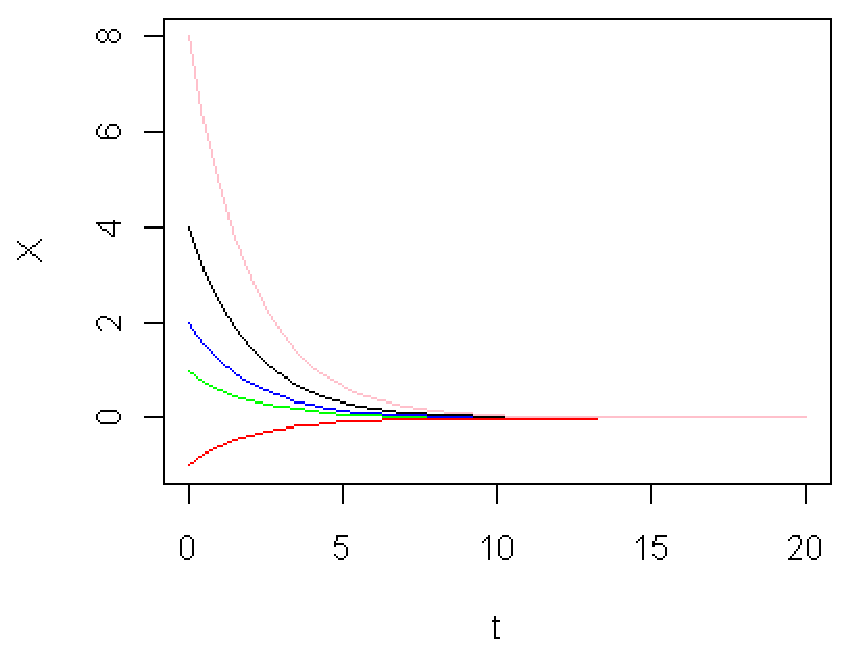
\includegraphics[height=6cm]{./images/gating_analytical.eps}}
  \caption{The family of $X=X(0)e^{-t/\tau}$ with $\tau=2$ and $X(0) =
    -1,1,2,4,8$}\label{fig:gating-analytical}
\end{figure}

To show how the initial value and setting parameters affect the shape
of the curves, in a data analysis, we need to use plots or graphics to
help readers understanding the problem easier. Here, we use
\hyperref[chap1.1.r]{R code} to plot the equation $X(t)$ with
\begin{itemize}
\item different initial values $X(0)$: (-1,1,2,4,8)

\item for a period of time from 0 to 20[unit of time], time step is
  0.5[unit of time].
\item Assuming that the mean open time $\tau$ (tau) is equal to 2ms.
\end{itemize}
\begin{equation}
  \label{eq:47}
  X = X(0) \times \exp({-t/\tau})
\end{equation}

In our example, the model of single type of channels describes
exponential decay (or growth) to a steady state fraction of open
channels, $f_\infty$, Fig.~\ref{fig:gating-analytical}.

{\bf Remarks:} The two important time points
\begin{itemize}
\item The time at which the value of the function decays to 1/2 of the
  initial value is called {\bf half-time},  denoted as $T_{1/2}$, with
  $T_{1/2} = \tau ln2$ since 
  \begin{equation}
    \label{eq:16}
    X(0) e^{-T_{1/2}/\tau} = \frac{X(0)}{2}
  \end{equation}
\item After a time period $t=\tau$, the value of X is $X = X(0)e^{-1}
  \approx X(0) \times 0.37$ (or the new value is e-fold decrease of
  the initial value)
\end{itemize}
The above principles apply to growing as well as decaying function in
the form of exponential. 


\subsection{Numerical solution}
\label{sec:numerical-solution-first-order-system}

Even though eq. \eqref{eq:255} has the exact solution; in many other ODE
formula, the analytical solution is rarely available. To solve the system on
computer, an approximation method is required in that the ODE needs to be
represented in the form of an algebraic equation that can be solved by the
computers.

This section will introduce how an approximated solution for an ODE can be
obtained.\footnote{For detailed references, read
  {\it Numerical methods for Engineers} - Chapra \& Canale.}
Sect.\ref{chap:ordin-diff-equat}) discusses more details different numerical
methods, depending upon the order of the ODE, and the level of accuracy in time
and/or space.

Using Taylor expansion (Sect.\ref{{sec:taylor-expansion}}), a simple method with
first-order accuracy in time (Sect.\ref{sec:numerical-method-ode-first-order})
is {\it Euler method}. The Euler method is identical to the first-order Taylor
expansion:
\begin{eqnarray*}
  X(t+\Delta t) = X(t) + \Delta t .X'(t)
\end{eqnarray*}
With $X'(t) = \frac{dX}{dt}=-\frac{X}{\tau}$, we have

\begin{equation}
  \label{eq:17}
  X(t + \Delta t) = X(t) - \frac{X(t)\Delta t}{\tau}
\end{equation}

Since  $X(\cdot) = f(\cdot) - f_\infty$, we have
\begin{equation}
  \label{eq:18}
  f(t+\Delta t) = f(t) - \frac{(f(t) - f_\infty)\Delta t}{\tau}
\end{equation}
Given this formula, by using an iterative approach, we can obtain the
value of the state function $f$ at a time instant $(t+\Delta t)$ given
the value of the state function at a previous time instant $t$.

\subsection{-- Example (R code)}
\label{sec:example-r-code}


\begin{figure}[htb]
  \centerline{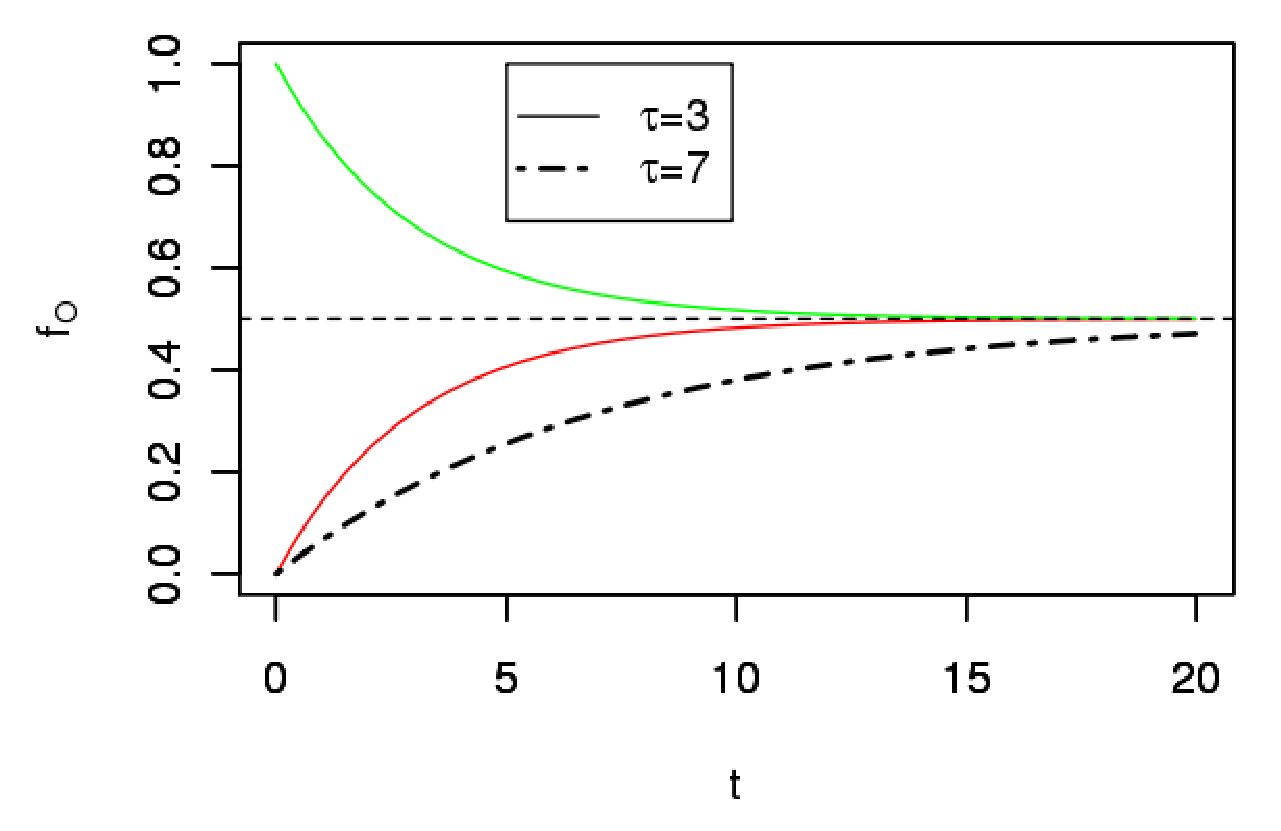
\includegraphics[height=6cm]{./images/gating_numerical.eps}}
  \caption{Analyze the dynamics of fraction opening channel
    $f=f(0)e^{-t/\tau}$ with $\tau=3$ms, 7ms, and $f(0) = 0$ and
    1}\label{fig:gating-numerical}
\end{figure}
Assuming that the time step is $\Delta t = 0.03$ms. We examine two
different initial conditions: (1) no channel is open($f(0) = 0$) and
(2) all channels are open ($f(0)=1$); as well as two time constants
$\tau = \{3, 7\}$ms. The steady-state fraction of open channel is
$f_\infty = 0.5$, as shown in Fig.~\ref{fig:gating-numerical}.

{\bf R-code}: (\hyperref[chap1.2.r]{chap1.2.r})

As shown in Fig. \ref{fig:gating-numerical}, the rate at which the
steady state is reached depends on the value of the time constant
$\tau$ (the smaller the $\tau$ or the faster the kinetics of the
gating mechanism).

\subsection{-- Example (in XPP)}
\label{sec:example-in-xpp}

A faster and easier way to analyze is using the XPP tool which has
many numerical methods installed, and visualization tool to see the
data. 
% \lstinputlisting{./codes/XPPAUT/chap1.}

\subsection{Analytical vs. Numerical solutions}
\label{sec:analyt-vs.-numer}

Let's see the difference between the results produced using the
analytical method and numerical methods, as given in
Fig.~\ref{fig:gating-comparison}
\begin{figure}[htb]
  \centerline{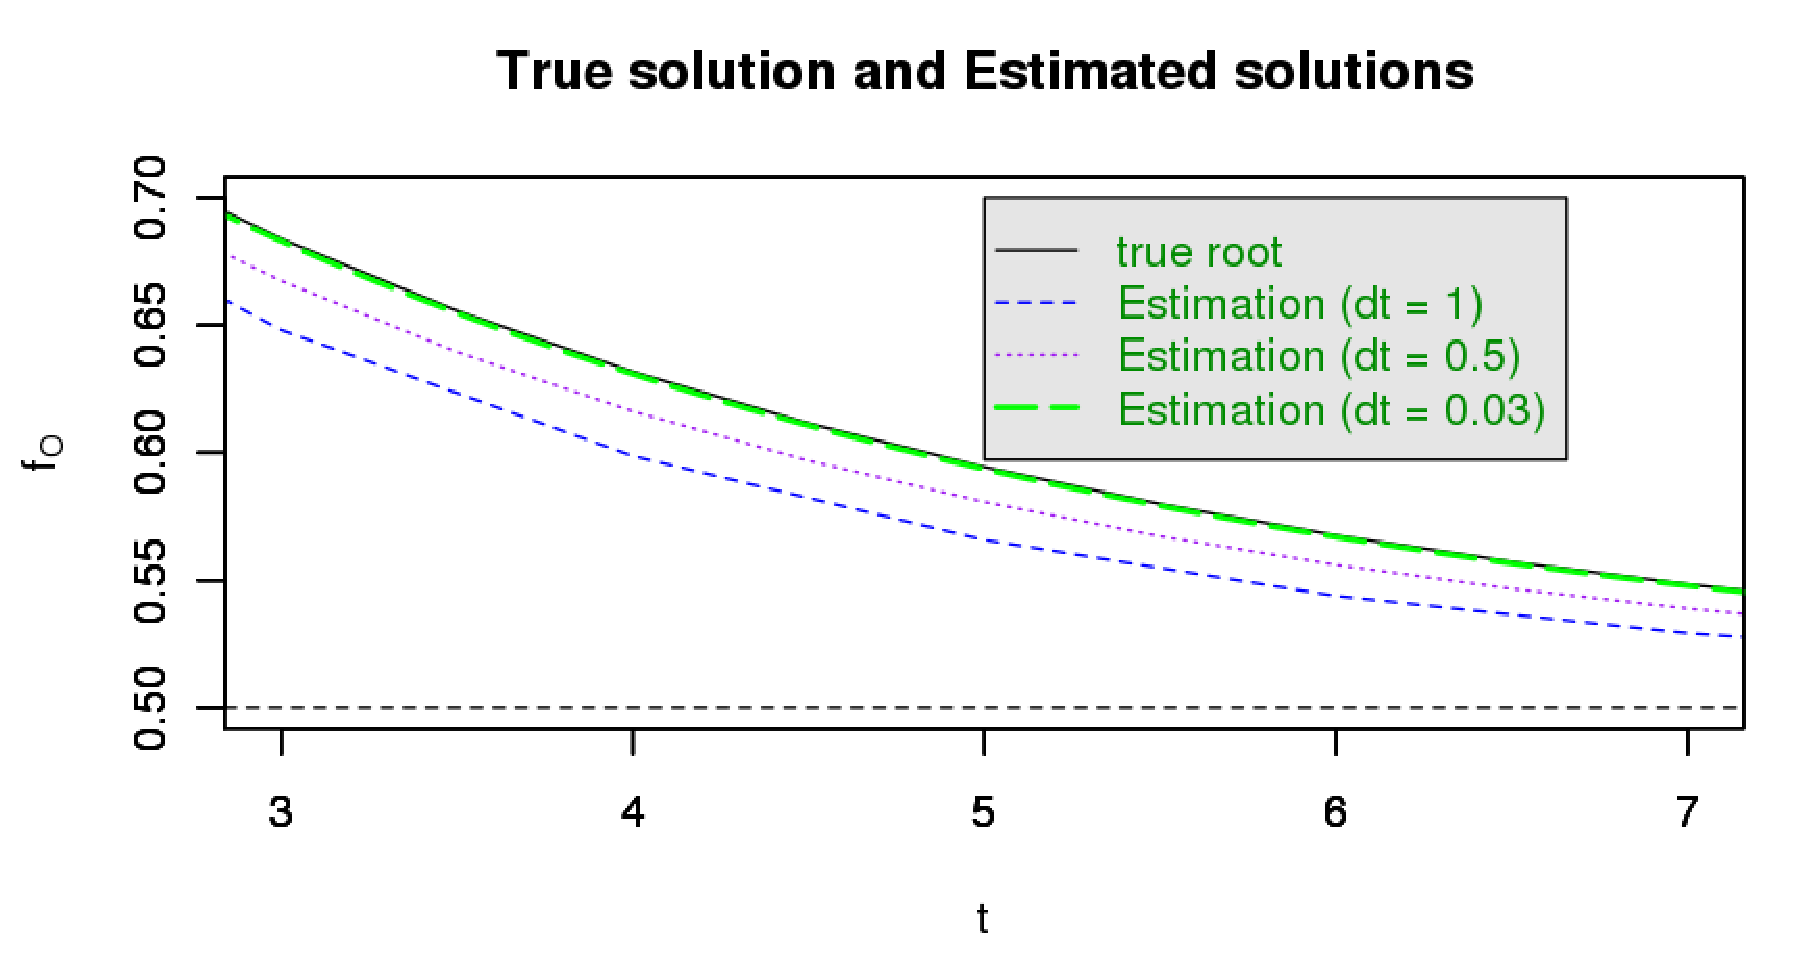
\includegraphics[height=7cm]{./images/gating_comparison.eps}}
  \caption{Approximated solution and analytical
    solutions}\label{fig:gating-comparison}
\end{figure}

{\bf Remarks:}

\begin{itemize}
\item The result of analytical method is always the true solution. All
  numerical methods just produce an approximated solution.

\item The accuracy of a numerical solution is highly dependent upon
  the selected parameters, e.g. the step size, as shown in
  Fig.~\ref{fig:gating-comparison}.  Only the step size whose
  {\it magnitude is smaller} than the value of $\tau$ do a reasonable
  job to approximate the exact exponential solution, e.g. $\Delta t =
  2 < \tau = 3$ is good, but $\Delta t = 6 > 3$ is
  bad.
  \textcolor{blue}{If we say an order of magnitude smaller/larger, it
    means 10x smaller/larger}.

\item There are different ways to plot the result of solving the
  differential equation that frequent gives insight into the
  properties of the solution.
\end{itemize}

{\bf R-code}: \hyperref[chap1.3.r]{chap1.3.r}

\subsection{Rate of change (phase diagram)}
\label{sec:analysis-rate-change}
\label{sec:rate-of-change-example}

Besides solving the dynamical system using analytical or numerical method, there
is a different way to study the system is by studying the {\it rate of change}
in time. 
\begin{enumerate}
  \item In the former approach, i.e. by plotting X or $f$ against the time $t$, we only
know change of the state function $f$ in the course of time.

  \item In the later approach, i.e. it is helpful to examine {\it how fast of
  the change}. Since the rate of change is indeed the first-order derivative of $f$,
we can plot $df/dt$ vs. $f$, without having to solve the ODE to find the exact
value of $f$.
\end{enumerate}

\begin{framed}

  A powerful mathematical tool to study the rate of change is {\bf phase plane
  analysis} (Sect.\ref{sec:phase-plane-analysis}).  This is particularly useful
  to analyze differential equations (ODE) with 2 variables. This will be covered
  in the next chapter.
\end{framed}

% \begin{equation} \label{eq:24} \frac{df}{dt} = \frac{f-f_\infty}{\tau} \text{ 
% vs.  } f \end{equation} tells us the rate of change as a function of $f$
% (portion of open channels).

\subsection{-- Example (R-code)}

{\bf R-code}: \hyperref[chap1.4.r]{chap1.4.r}

\begin{figure}[htb]
  \centerline{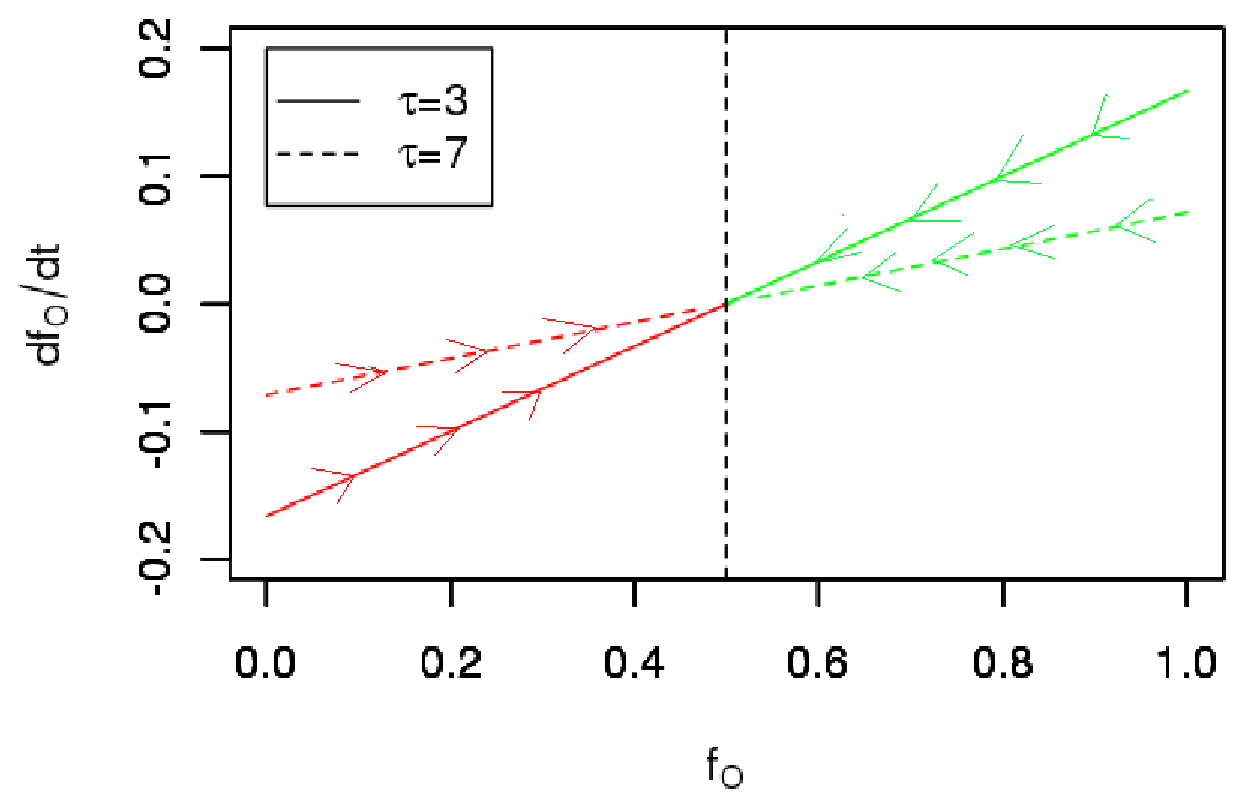
\includegraphics[height=7cm]{./images/gating_rate.eps}}
  \caption{Rate of open state-transient at different mean open time
    constant. $f =\frac{N_0}{N}$ is restricted within [0,1] on
    physical background}\label{fig:gating-rate}
\end{figure}

Given $f_\infty = 0.5$ and two initial conditions: $f_0 = 0$ or 1, the
plot in Fig. \ref{fig:gating-rate} shows that all converge to the
steady-state fraction open channel $f_\infty$.  The steeper the line,
the faster the rate of opening the channels $df/dt$; the lower the
value of mean open time constant $\tau$; the faster the
opening-transient of the channels.  

With two different initial fraction opening channels, both converge to
the same steady state fraction opening channels $f_\infty$. Thus, to
show the direction of the change, we can use the arrow to show the
direction in which $f$ is changing. 

{\bf Remarks:} 
\begin{itemize}
\item When analyzing the gating phenomena, in a cell, there are
  thousands of ion channels of a given type. Then, a reasonable way is
  to study the average behavior of the entire ensemble of channels (or
  in some circumstances, a local region) to determine the {\bf
    cellular dynamics}.
\end{itemize}

\subsection{Steady-state value and time-constant}

From the given example, there are two quantities of a variable X that follows
first-order kinetics that we will see again, and very often. They are 
\begin{itemize}
  \item stead-state value $X_\infty$
  \item time constant $\tau_X$
\end{itemize}

% Another and better notation is to define
\begin{equation}
  \label{eq:685}
  \begin{split}
f_\infty=\frac{k^+}{k^-+k^+} \\
\tau=\frac{1}{k^-+k^+}
\end{split}
\end{equation}

So, we have
\begin{equation}
  \label{eq:686}
  \frac{df}{dt} = -\frac{f-f_\infty}{\tau}
\end{equation}
We easily realize that $f_\infty$ is the value of $f$ at steady-state,
i.e. when $df/dt=0$, and $\tau$ is the time it takes for X to change from
initial value to the a new value that is $1/e$ times the initial value (for
decay) or $e$ times the initial value (for increase).
% mean of the distribution.
% More detail will be given in the next chapter.
%   Denote $x = f_0(t)$ as the number of open channels at a given time
%   point that depend on $t$.  Clearly, this is a differential
%   equation
%   \begin{equation}
%     \label{eq:12}
%     \frac{dx}{dt} = -\frac{x-k}{\tau}
%   \end{equation}
%   with
%   \begin{equation}
%     \label{eq:150}
%     \tau = \frac{1}{k^++k^-}; k=\frac{k^+}{k^++k^-}
%   \end{equation}
% \item What remains are the analysis of the eq. \eqref{eq:12}.
  
%   Eq. \eqref{eq:12} has the form of a simple linear equation
%   \begin{equation}
%     \label{eq:13}
%     \frac{dX}{dt} = -\frac{X}{\tau}
%   \end{equation}
%   with $X = x - k = f_0(t) - k$.

\section{Summary}
\label{sec:summary-7}

In this chapter, you have learnt a general procedure to develop a model, with a
sample of modeling the dynamics of a system of 2-state ionic channels. We also
learnt important concepts being used in modelling. In the next chapter, we will
discuss in detail ionic channels, and how to model their kinetics in an
excitable cell.

%%% Local Variables: 
%%% mode: latex
%%% TeX-master: "mainfile"
%%% End: 
